\documentclass[border=2mm,12pt,tikz]{standalone}
\usepackage{tikz-3dplot} 
\usepackage{bm}
\usetikzlibrary{intersections,patterns.meta}
\begin{document}
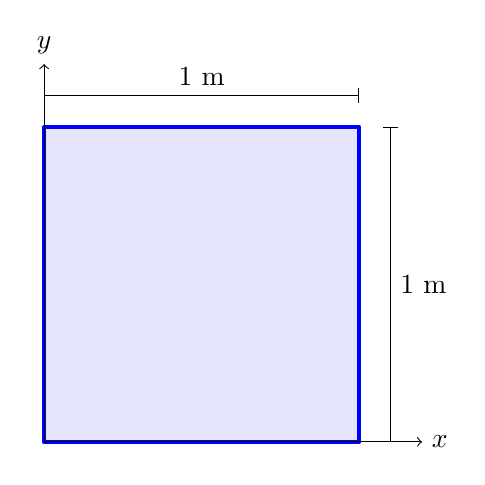
\begin{tikzpicture}[
        scale = 4, 
        line join=round,
        mystyle/.style = {ultra thick, blue, fill=blue!20, fill opacity=0.5}
    ]

    \coordinate (1) at (0,0);
    \coordinate (2) at (1,0);
    \coordinate (3) at (0,1);
    \coordinate (4) at (1,1);

    \draw[mystyle] (1) -- (2) -- (4) -- (3) -- cycle;


    \draw[->] (0, 0, 0) -- (1.2, 0, 0) node[right] {$x$};
    \draw[->] (0, 0, 0) -- (0, 1.2, 0) node[above] {$y$};

    \draw[|-|] (3) ++ (0, 0.1) --++ (1,0) node[midway, above] {$1$ m};
    \draw[|-|] (4) ++ (0.1,0) --++ (0,-1) node[midway, right] {$1$ m};
    % \draw[|-|] (2) ++ (0, 0, 0.1) --++ (0,1,0) node[midway, right] {$1$ m};
    % \draw[|-|] (5) ++ (0, 0, 0.1) --++ (1,0,0) node[midway, right] {$1$ m};
\end{tikzpicture}
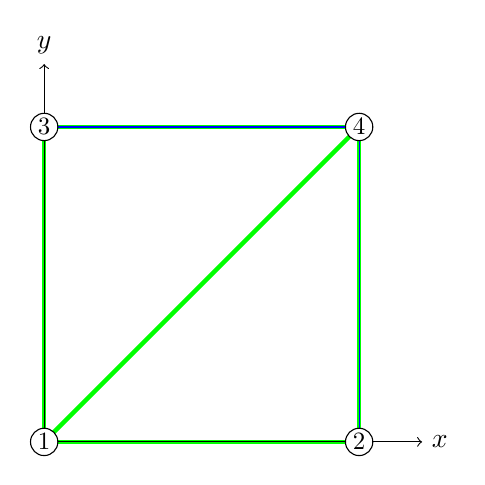
\begin{tikzpicture}[
        scale = 4, 
        line join=round,
        mystyle/.style = {ultra thick, green},
        mystyle2/.style = {blue}
    ]
        \coordinate (1) at (0,0);
        \coordinate (2) at (1,0);
        \coordinate (3) at (0,1);
        \coordinate (4) at (1,1);


        \draw[mystyle] (1) -- (2) -- (4) -- (3) -- cycle;
        \draw[mystyle] (1) -- (4);
        \draw[mystyle2] (1) -- (2) -- (4) -- (3) -- cycle;


        \draw[->] (0, 0, 0) -- (1.2, 0, 0) node[right] {$x$};
        \draw[->] (0, 0, 0) -- (0, 1.2, 0) node[above] {$y$};

        \draw (1) node[ circle, draw, inner sep=1pt, fill=white, thin, scale = 0.9, fill opacity = 1] {$1$};
        \draw (2) node[ circle, draw, inner sep=1pt, fill=white, thin, scale = 0.9, fill opacity = 1] {$2$};
        \draw (3) node[ circle, draw, inner sep=1pt, fill=white, thin, scale = 0.9, fill opacity = 1] {$3$};
        \draw (4) node[ circle, draw, inner sep=1pt, fill=white, thin, scale = 0.9, fill opacity = 1] {$4$};

    \end{tikzpicture}
    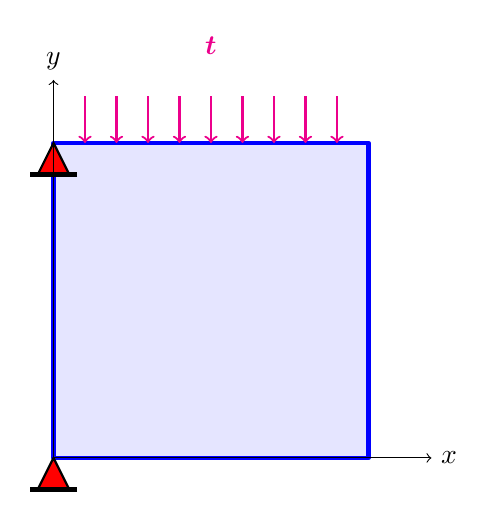
\begin{tikzpicture}[
        scale = 4, 
        line join=round,
        mystyle/.style = {ultra thick, blue, fill=blue!20, fill opacity=0.5}
    ]

        \coordinate (1) at (0,0);
        \coordinate (2) at (1,0);
        \coordinate (3) at (0,1);
        \coordinate (4) at (1,1);

    \draw[mystyle] (1) -- (2) -- (4) -- (3) -- cycle;

    \draw[thick, fill = red] (1) --++ (0.05, -0.1, 0) --++ (-0.1, 0, 0) -- cycle;
    \draw[ultra thick] (1) ++ (0.075, -0.1, 0) --++ (-0.15, 0, 0);
    \draw[thick, fill = red] (3) --++ (0.05, -0.1, 0) --++ (-0.1, 0, 0) -- cycle;
    \draw[ultra thick] (3) ++ (0.075, -0.1, 0) --++ (-0.15, 0, 0);


    \draw[->] (0, 0, 0) -- (1.2, 0, 0) node[right] {$x$};
    \draw[->] (0, 0, 0) -- (0, 1.2, 0) node[above] {$y$};


    \foreach \x in {0.1, 0.2, ..., 0.9} {
        \draw[<-, magenta, thick] (\x, 1) --++ (0, 0.15);
    }

    \draw (0.5, 1.25) node[above, magenta] {$\bm{t}$};

\end{tikzpicture}
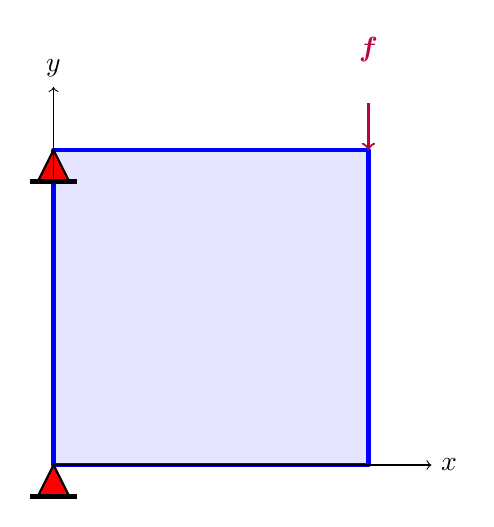
\begin{tikzpicture}[
    scale = 4, 
    line join=round,
    mystyle/.style = {ultra thick, blue, fill=blue!20, fill opacity=0.5}
]
    \coordinate (1) at (0,0);
    \coordinate (2) at (1,0);
    \coordinate (3) at (0,1);
    \coordinate (4) at (1,1);

    \draw[mystyle] (1) -- (2) -- (4) -- (3) -- cycle;

    \draw[thick, fill = red] (1) --++ (0.05, -0.1, 0) --++ (-0.1, 0, 0) -- cycle;
    \draw[ultra thick] (1) ++ (0.075, -0.1, 0) --++ (-0.15, 0, 0);
    \draw[thick, fill = red] (3) --++ (0.05, -0.1, 0) --++ (-0.1, 0, 0) -- cycle;
    \draw[ultra thick] (3) ++ (0.075, -0.1, 0) --++ (-0.15, 0, 0);


    \draw[->] (0, 0, 0) -- (1.2, 0, 0) node[right] {$x$};
    \draw[->] (0, 0, 0) -- (0, 1.2, 0) node[above] {$y$};


    \draw[<-, purple, thick] (4) --++ (0, 0.15);

    \draw (4) ++ (0,0.25) node[above, purple] {$\bm{f}$};

\end{tikzpicture}
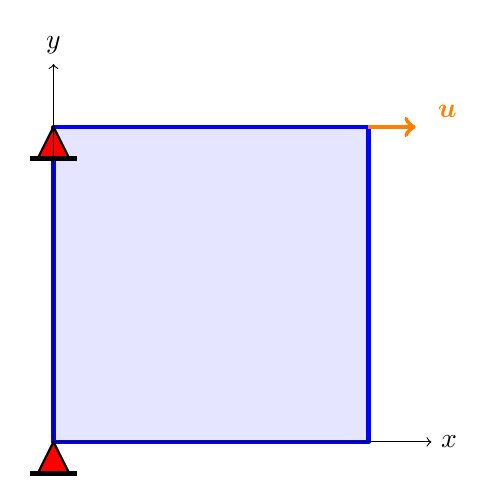
\begin{tikzpicture}[
    scale = 4, 
    line join=round,
    mystyle/.style = {ultra thick, blue, fill=blue!20, fill opacity=0.5}
]

\coordinate (1) at (0,0);
\coordinate (2) at (1,0);
\coordinate (3) at (0,1);
\coordinate (4) at (1,1);

\draw[mystyle] (1) -- (2) -- (4) -- (3) -- cycle;

\draw[thick, fill = red] (1) --++ (0.05, -0.1, 0) --++ (-0.1, 0, 0) -- cycle;
\draw[ultra thick] (1) ++ (0.075, -0.1, 0) --++ (-0.15, 0, 0);
\draw[thick, fill = red] (3) --++ (0.05, -0.1, 0) --++ (-0.1, 0, 0) -- cycle;
\draw[ultra thick] (3) ++ (0.075, -0.1, 0) --++ (-0.15, 0, 0);


\draw[->] (0, 0, 0) -- (1.2, 0, 0) node[right] {$x$};
\draw[->] (0, 0, 0) -- (0, 1.2, 0) node[above] {$y$};


\draw[->, orange, ultra thick] (4) --++ (0.15, 0);

\draw (4) ++ (0.25,0) node[above, orange] {$\bm{u}$};


\end{tikzpicture}
\end{document} 